% Modle pour rapport de Travail de Fin d'Etudes de l'Ecole Centrale de Lyon
% version 0.1
% 2009-07-24
% par Steren Giannini (steren.giannini@gmail.com)
% Ce modèle est mis  disposition selon le Contrat "Creative Commons
% Paternité-Partage des Conditions Initiales  l'Identique 3.0 Unported"
% http://creativecommons.org/licenses/by/3.0/
\documentclass[12pt]{article}
%Chargement des packages
\usepackage[utf8]{inputenc}
\usepackage[french]{babel} %le rapport est en français 
\usepackage{amsmath}
\usepackage{amsfonts}
\usepackage{amssymb}
\usepackage{graphicx} %pour afficher des images
\usepackage{float}    %pour forcer le placement des images.
\usepackage{geometry} %pour la modification des marges
\usepackage{fancyhdr} %pour modification des pieds de page
\usepackage{longtable}
\usepackage{listings}
\usepackage{subfigure}
\usepackage{hyperref} %pour que les références soient des liens hypertextes
\usepackage[usenames,dvipsnames]{color} % pour les textes en gris


% Comment utiliser :
% - la page de titre est à personnaliser (title/title.tex)
% - le contenu est à rédiger dans le répertoire pages/, s'inspirer des exemples
%   présents dans ce modèle.
% - les annexes sont à rédiger dans le répertoire appendix/
% - la bibliographie utilise BibTex (fichier biblio.bib)
% - les variables suivantes sont à remplir :
\newcommand{\TitreRapport}{Rassemblement d'agents mobiles}
\newcommand{\DateRapport}{Mai 2014}
\newcommand{\AuteurRapport}{Eloi Perdereau}

%définition des marges
\geometry{margin=2cm}

%utilisation des puces anglaises.
%attention, il faut avoir une version récente de frenchb.ldf.
\frenchbsetup{StandardItemLabels}

%Définition des en-têtes et pieds de page
\renewcommand{\headrulewidth}{0pt}
\renewcommand{\footrulewidth}{0.5pt}
% \fancyhead[L]{{\small\TitreRapport}}
\fancyfoot[C]{\small\TitreRapport}
\fancyfoot[L]{\small\AuteurRapport}
\fancyfoot[R]{\thepage}

% définition du titre, de la date et de l'auteur du document
\title{\TitreRapport}
\date{\DateRapport}
\author{\AuteurRapport}

\makeatletter

\renewcommand\maketitle{
  \begin{titlepage}
    \begin{center}
      
\includegraphics[width=7.2cm]{title/images/logo_AMU.png}
      \hspace{\stretch{1}}
      
\includegraphics[width=7.2cm]{title/images/logo_LIF.png}

    \vspace{\stretch{0.2}}

      \begin{tabular*}{1.0\textwidth}{l @{\extracolsep{\fill}} r}
          Département Informatique et Interactions & \NomEntreprise \\
          TER \@date                               & Marseille      \\
      \end{tabular*}

    \vspace{\stretch{1.5}}

      {\large \bf Rapport de Travail Encadré de Recherche \\}
      \vspace{0.5cm}
      {\LARGE \bf \@title\\}
      \vspace{0.5cm}
      {\large \it \@author\\}

    \vspace{\stretch{2}}
      
\includegraphics[width=1.0\textwidth]{title/images/logo_illustration.png}
    \vspace{\stretch{2}}

      \begin{tabular}{rl}
        \textit{Tuteur}~:          & Shantanu Das  \\
        \textit{Responsable TER}~: & Omar Boucelma \\
      \end{tabular}

%       \begin{tabular*}{1.0\textwidth}{|l @{\extracolsep{\fill}} r|}
%         \hline
%           Tuteurs :             & Option : (sigle développé)  \\
%           &\\
%           \textit{ECL} :        &                             \\
%           Nom, Prénom Tuteur 1  & Filière : (sigle développé) \\
%           Nom, Prénom Tuteur 2  &                             \\
%           &\\
%           \textit{Entreprise} : &                             \\
%           Nom, Prénom Tuteur 1  & Métier : (sigle développé)    \\
%           Nom, Prénom Tuteur 2  &                             \\
%         \hline
%       \end{tabular*}

    \end{center}\par

  \end{titlepage}
  \setcounter{footnote}{0}
}

\makeatother

\usetikzlibrary{calc}   % coordinate calculation

\newcommand{\defstuff} {
  \def \step {1}
  \def \cc {\step/2}  % center of cell
  \coordinate (offset) at ($(\cc,\cc)$);
}

\newcommand{\drawgrid}[1] {
  \draw[step=\step, color=gray] (0,0) grid ($#1$); % draw the grid, base at #1
}

\newcommand{\drawrobots}[1] {
    \foreach \coord in #1 {
      \coordinate[at=\coord, name=A];
      \draw ($(A) + (offset)$) circle ({\cc*0.8});
    }
}

\newcommand{\drawarrows}[1] {
    \foreach \a/\b in #1 {
      \coordinate[at=\a, name=A];
      \coordinate[at=\b, name=B];
      \draw[->, color=darkgray] ($(A) + (offset)$) -- ($(B) + (offset)$);
    }
}

\newcommand{\spacee}[3] {
  \begin{tikzpicture}[thick, scale=0.6]
    \defstuff
    \drawgrid{#1}
    \drawrobots{#2}
    \drawarrows{#3}
  \end{tikzpicture}
}


\newcommand{\GatheringProblem}{\ensuremath{\textsc{Gathering Problem}}\xspace}

\begin{document}
\pagestyle{fancy}

\maketitle
    \newpage
\section*{Remerciements}

Je tiens à remercier mon tuteur, Mr Shantanu Das qui m'a été d'une aide
précieuse tout au long du projet, en m'accordant son temps et en m'apportant
ses connaissances et son expérience du monde de la recherche.

    \newpage
\tableofcontents
    \newpage
\section*{Introduction}
\addcontentsline{toc}{section}{Introduction}
Dans le cadre de ma première année de Master informatique à Aix-Marseille
Univsersité (site de Luminy), je suis amené à faire un projet (TER) encadré par
un chercheur d'AMU ou un stage en entreprise. Ayant plus une vocation liée à la
recherche, je me suis orienté vers un projet mêlant programmation et théorie
fondamentale. \\

Le projet rentre dans le domaine de l'algorithmique distribuée~; branche de
l'informatique théorique dont le but est de développer des algorithmes pour des
systèmes distribués impliquant plusieurs processus interconnectés par un
réseau. Ces processus indépendants interagissent et coopèrent entre eux en vue
de réaliser une tâche donnée.  L'idée principal du calcul distribué est que les
processus communiquent entre eux par l'envoi de messages. Néanmoins, nous nous
intéressons ici à un paradigme légèrement différent : les \textit{agents
mobiles}. Ce sont des programmes qui peuvent se déplacer de n\oe{}uds en
n\oe{}uds à l'intérieur du réseau de manière autonome. Bien qu'ils peuvent être
implémentés via le modèle précédent (et font donc parti du calcul distribué),
ils fournissent une abstraction plutôt naturelle pour le développement
d'algorithmes tels que la détection d'intrus, l'exploration d'un réseau
inconnu, ou encore la formation d'un motif par des robots (\textit{robot
pattern formation problem}). Ce dernier problème consiste à arranger les robots
dans le plan pour qu'ils forment et conservent un motif donné. \\

L'objectif ici est de développer et d'implémenter une solution pour un cas
particulier de ce problème~: le rassemblement d'agents mobiles. Aussi appelé le
\GatheringProblem, beaucoup de contributions y ont déjà été apporté, impliquant
souvent un plan continu ou une visibilité infinie. Nous nous restreignons ici à
un espace discret et une visibilité constante des robots. De plus, le système
est synchrone, c'est à dire qu'il existe une horloge globale partagée par tous
les processus. Autrement dit, les algorithmes fonctionneront par
\textit{rondes} (ou \textit{étapes}.) Pour notre cas, cela signifie que tous
les robots décident et se déplacent en même temps.

Le travail à réaliser dans ce projet est donc la recherche des cas de voisinage
et de déplacement des robots pour le \GatheringProblem dans notre contexte. Il
faut également développer une application permettant la visualisation des
robots et de l'algorithme distribué. Cette partie sera faite en utilisant le
langage Python et la librairie TKinter pour l'interface graphique. \\

Dans un premier temps je vais vous présenter plus en détail le sujet et les
outils utilisés~; puis je vous exposerais le travail que j'ai réalisé
développant les différentes étapes de recherche d'un algorithme correct ainsi
que les techniques d'implémentation utilisés. Enfin, je conclurai par un bilan
personnel et professionnel.

    % \newpage
% \listoffigures
% \listoftables
    \newpage
\newcommand{\Observer}{\textit{Observer}\xspace}
\newcommand{\Calculer}{\textit{Calculer}\xspace}
\newcommand{\SeDeplacer}{\textit{Se\_déplacer}\xspace}

\section{Cadre du projet}

\subsection{Présentation du sujet}

Bien que le problème ne soit théorique, nous modélisons un système plus ou
moins réaliste qui pourrait émerger d'applications pratiques. Néanmoins, nous
allons nous concentrer sur le développement d'un algorithme correct pour
résoudre le problème posé sans se soucier des cas pratiques.

Comme énoncé dans l'introduction, nous nous plaçons dans le cadre d'un univers
discret. C'est à dire que le plan peut être représenté par un graphe simple
non-orienté où chaque sommet possède 8 voisins différentiables par leur
coordonnées relatives au sommet considéré. Les entités mobiles (ou robots) sont
modélisés comme des unités de calcul ayant une mémoire locale et sont capables
d'effectuer des calculs locaux. Les robots sont placés dans le plan et sont
représentés par des points de $\mathbb{N}^2$. Ils sont capables de se déplacer
librement dans l'espace de manière synchrone et sont dotés de capacités
sensorielles leur permettant d'observer la position de leur voisin à un instant
$t$. Plus formellement, les robots effectuent en permanence une succession de
trois opérations~:
\begin{enumerate}[(i)]
  \item \Observer. Le robot observe son voisinage en activant ses
  capteurs qui lui renvoient un instantané des positions des robots à
  l'intérieur de son champ de visibilité.
  \item \Calculer. Le robot effectue un calcul local donné par
  l'algorithme. Le résultat de ce calcul est un point de destination (à
  distance au plus 1 du robot concerné). Si ce point est la position du robot,
  celui-ci ne se déplace pas.
  \item \SeDeplacer. Le robot se déplace à la position renvoyée par le
  calcul. \\
\end{enumerate}
La séquence \Observer-\Calculer-\SeDeplacer constitue un cycle de calcul. On
définit plusieurs contraintes et suppositions sur les robots dont il faut nous
soumettre.

\paragraph{Synchronicité} Le temps passé pour \Observer, \Calculer et
\SeDeplacer est le même pour tous les robots. De plus, ils commencent à
\Observer en même temps.

\paragraph{Pas de communication directe entre les robots} Certains modèles
permettent l'envoi de messages entre les robots en plus de leur déplacement.
Cela est en effet assez réaliste si les robots sont considérés sont des
machines électroniques avec des capacités de communications et un protocole
défini. Néanmoins, nous n'autorisons ici qu'une communication indirecte avec
leur positions relatives.

\paragraph{Visibilité limitée} Les robots ne sont capables de recevoir de leur
capteurs uniquement des informations sur leur entourage restreint. Ils n'ont
donc pas de connaissance du nombre total de robots où de la présence de robots
en dehors de leur champ de visibilité (\textit{visibility radius}.)

\paragraph{Homogénéité} Tous les robots sont pré-programmés avec un même
algorithme et commencent à la même étape. Le système étant synchrone, ils
peuvent garder localement un compteur de cycle qu'ils effectuent, et ce
compteur aura la même valeur pour tous les robots à chaque instant de
l'algorithme.

\paragraph{Anonymat} Il n'existe aucun paramètre global permettant de dissocier
les robots. Leur capteurs leur renvoie donc que des informations sur la
position des robots alentours, et nullement des particularités propres à chaque
robot voisin.

\paragraph{Points denses} Plusieurs robots peuvent se retrouver dans une même
position a un instant $t$. Il n'est pas nécessaires pour un robot de connaitre
le nombre de robots sur un point particulier, car une fois qu'ils sont à la
même position, tous recevrons les mêmes informations de leur capteurs, et
prendrons donc la même décision du fait de leur homogénéité. On peut donc les
considérer comme un seul robot.

\paragraph{Mémoire constante} Chaque robot ne peut retenir en mémoire qu'un
nombre limité d'informations. Par exemple, son dernier mouvement ou son
entourage précédent.

\paragraph{Déplacement 1} \`A chaque étape, les robots ne peuvent se déplacer que
sur un n\oe{}ud voisin direct.

\paragraph{Désorientation} En plus d'avoir un système de coordonnée différente,
les robots ont également leur propre orientation. Nous ne pouvons donc pas nous
fier à l'orientation des instantanés reçues sur les entourages et devons les
considérer comme s'ils avaient subies aléatoirement des rotations successives
des $90^{\circ}$.

\paragraph{Autonomie} Le mécanisme de coordination utilisé par les robots pour
se rassembler doit être totalement décentralisé, i.e aucun contrôle central
n'est utilisé.

\paragraph{Terminaison} Du fait de l'autonomie des robots~: à la fin de chaque
étape, chaque robot doit savoir s'il est dans un état terminal ou non. Il n'y a
donc pas de système global permettant la désactivation des robots à distance.
Quand tous les robots sont dans un état terminal, ils s'arrêtent et
l'algorithme se termine. Quand aucun robot ne se déplace lors d'une étape, le
système n'évoluera plus~; on dit qu'on a atteint un état quescient. \\

Le graphe défini comme sous graphe de l'espace ne contenant que les n\oe{}uds
occupés par des robots est connexe au départ, et doit le rester après chaque
cycle. C'est à dire que chaque robot est accessible par tous les autres en ne
passant que par des robots à distance 1. Cette restriction est nécessaire car,
intuitivement, il est très difficile, voire impossible pour un robot qui n'a
pas de voisin de se rassembler avec les autres robots de l'espace dû à sa
visibilité limitée. On peut dire qu'on a un point de rassemblement par
composante connexe.

Concernant ce point de rassemblement, on ne peut pas garantir son unicité à
cause de la désorientation des robots. Par exemple, s'il ne reste que deux
robots adjacents, ils ont le même voisinage (à une rotation près), et donc il
n'y a pas moyen de les dissocier pour choisir un point unique pour le
rassemblement. Nous considérons donc que s'il y a 1, 2 ou 4 robots adjacents,
l'algorithme peut se terminer et les robots sont rassemblés. Plus précisément,
les cas de terminaison sont exposés en figure \ref{fig:end_cases}.
\begin{figure}[h!]
  \centering
  \begin{subfigure}[b]{0.16\textwidth}
    \resizebox{\linewidth}{!} {
      \spacee {(3,3)} {{(1,1)}} {{}}
    }
  \end{subfigure}
  \begin{subfigure}[b]{0.20\textwidth}
    \resizebox{\linewidth}{!} {
      \spacee {(4,3)} {{(1,1),(2,1)}} {{}}
    }
  \end{subfigure}
  \begin{subfigure}[b]{0.20\textwidth}
    \resizebox{\linewidth}{!} {
      \spacee {(4,4)} {{(1,1),(2,2)}} {{}}
    }
  \end{subfigure}
  \begin{subfigure}[b]{0.20\textwidth}
    \resizebox{\linewidth}{!} {
      \spacee {(4,4)} {{(1,1),(2,1),(1,2),(2,2)}} {{}}
    }
  \end{subfigure}
\caption{Cas terminaux globaux}
\label{fig:end_cases}
\end{figure}




\subsection{Déroulement du projet}
TODO \\
Le projet est fait seul, et j'utilise un système de gestion de version (Git)
hébergé par Github. Cela me permet d'avoir les sources et toute l'historique de
mon travail où que je sois, et cela rend la communication avec mon tuteur plus
simple, il peut voir le travail que je réalise à tout moment.
\LaTeX -> plaintext -> suivi des modifications des documents.
python tkinter \\

    \newpage
\section{Travail réalisé}

Cette section retrace le travail que j'ai réalisé durant ce projet, les
difficultés que j'ai rencontré ainsi que les solutions apportées.

\subsection{Recherche fondamentale}

Le processus de recherche a nécessité plusieurs étapes, et est encore en cours.
Dans un premier temps, il a fallu déterminer les cas de voisinage (instantanés)
dans lesquels les robots effectuent un mouvement. On considère d'abord que les
robots n'ont qu'une visibilité de 1, c'est à dire qu'ils ne voient que les
robots qui sont dans des cellules adjacentes. La figure \ref{fig:cas} en annexe
montre tous les cas de voisinage à distance 1 qu'un robot peut rencontrer. Il
n'est pas nécessaire de traiter les cas analogues correspondant à des rotations
de $90^\circ{}$, $180^\circ{}$ et $270^\circ{}$ de chacun de ces cas.  En
effet, lorsqu'un robot reçoit un instantané qui ne fait pas parti des cas
exposés, il effectue la rotation nécessaire, et applique l'algorithme selon le
cas ayant subi la rotation. \\

L'idée de base pour le rassemblement est d'\textit{arrondir les angles}. La
figure \ref{fig:cas_mvt} montre les cas sujet à mouvements.

\begin{figure}
  \centering
  % \captionsetup[subfigure]{labelformat=empty}
  \begin{subfigure}[b]{0.15\textwidth}
    \resizebox{\linewidth}{!} {
      \spacee {(3,3)} {{(1,1),(2,0)}}                   {{{(1,1)/(2,0)}}}
    }
    \caption{}
  \end{subfigure}
  \begin{subfigure}[b]{0.15\textwidth}
    \resizebox{\linewidth}{!} {
      \spacee {(3,3)} {{(1,1),(1,0)}}                   {{{(1,1)/(1,0)}}}
    }
    \caption{}
  \end{subfigure}
  \begin{subfigure}[b]{0.15\textwidth}
    \resizebox{\linewidth}{!} {
      \spacee {(3,3)} {{(1,1),(2,0),(1,0)}}             {{{(1,1)/(1,0)}}}
    }
    \caption{}
  \end{subfigure}
  \begin{subfigure}[b]{0.15\textwidth}
    \resizebox{\linewidth}{!} {
      \spacee {(3,3)} {{(1,1),(0,0),(2,0)}}             {{{(1,1)/(1,0)}}}
    }
    \caption{}
  \end{subfigure}
  \begin{subfigure}[b]{0.15\textwidth}
    \resizebox{\linewidth}{!} {
      \spacee {(3,3)} {{(1,1),(0,0),(1,0)}}             {{{(1,1)/(1,0)}}}
    }
    \caption{}
  \end{subfigure}
  \begin{subfigure}[b]{0.15\textwidth}
    \resizebox{\linewidth}{!} {
      \spacee {(3,3)} {{(1,1),(0,0),(2,1)}}             {{{(1,1)/(1,0)}}}
    }
    \caption{}
  \end{subfigure}
  \begin{subfigure}[b]{0.15\textwidth}
    \resizebox{\linewidth}{!} {
      \spacee {(3,3)} {{(1,1),(2,0),(0,1)}}             {{{(1,1)/(1,0)}}}
    }
    \caption{}
  \end{subfigure}
  \begin{subfigure}[b]{0.15\textwidth}
    \resizebox{\linewidth}{!} {
      \spacee {(3,3)} {{(1,1),(0,1),(1,0)}}             {{{(1,1)/(0,0)}}}
    }
    \caption{}
  \end{subfigure}
  \begin{subfigure}[b]{0.15\textwidth}
    \resizebox{\linewidth}{!} {
      \spacee {(3,3)} {{(1,1),(0,0),(1,0),(2,0)}}       {{{(1,1)/(1,0)}}}
    }
    \caption{}
  \end{subfigure}
  \begin{subfigure}[b]{0.15\textwidth}
    \resizebox{\linewidth}{!} {
      \spacee {(3,3)} {{(1,1),(2,0),(1,0),(2,1)}}       {{{(1,1)/(1,0)}}}
    }
    \caption{}
  \end{subfigure}
  \begin{subfigure}[b]{0.15\textwidth}
    \resizebox{\linewidth}{!} {
      \spacee {(3,3)} {{(1,1),(0,0),(1,0),(2,1)}}       {{{(1,1)/(1,0)}}}
    }
    \caption{}
  \end{subfigure}
  \begin{subfigure}[b]{0.15\textwidth}
    \resizebox{\linewidth}{!} {
      \spacee {(3,3)} {{(1,1),(2,0),(1,0),(0,1)}}       {{{(1,1)/(1,0)}}}
    }
    \caption{}
  \end{subfigure}
  \begin{subfigure}[b]{0.15\textwidth}
    \resizebox{\linewidth}{!} {
      \spacee {(3,3)} {{(1,1),(0,0),(2,1),(2,2)}}       {{{(1,1)/(1,0)}}}
    }
    \caption{}
  \end{subfigure}
  \begin{subfigure}[b]{0.15\textwidth}
    \resizebox{\linewidth}{!} {
      \spacee {(3,3)} {{(1,1),(2,0),(0,1),(0,2)}}       {{{(1,1)/(1,0)}}}
    }
    \caption{}
  \end{subfigure}
  \begin{subfigure}[b]{0.15\textwidth}
    \resizebox{\linewidth}{!} {
      \spacee {(3,3)} {{(1,1),(0,0),(2,1),(2,0)}}       {{{(1,1)/(1,0)}}}
    }
    \caption{}
  \end{subfigure}
  \begin{subfigure}[b]{0.15\textwidth}
    \resizebox{\linewidth}{!} {
      \spacee {(3,3)} {{(1,1),(0,0),(0,1),(2,0)}}       {{{(1,1)/(1,0)}}}
    }
    \caption{}
  \end{subfigure}
  \begin{subfigure}[b]{0.15\textwidth}
    \resizebox{\linewidth}{!} {
      \spacee {(3,3)} {{(1,1),(0,0),(1,0),(2,0),(2,1)}} {{{(1,1)/(1,0)}}}
    }
    \caption{}
  \end{subfigure}
  \begin{subfigure}[b]{0.15\textwidth}
    \resizebox{\linewidth}{!} {
      \spacee {(3,3)} {{(1,1),(0,0),(1,0),(2,0),(0,1)}} {{{(1,1)/(1,0)}}}
    }
    \caption{}
  \end{subfigure}
\caption{Cas de voisinnage sujet à mouvement}
\end{figure}



Ces cas semblent assez naturels, cependant ce n'est pas aussi simple. Par
exemple, examinons de plus près les cas (f) et (g). Si les robots se déplacent
dans ces cas, il existe une infinité d'arrangements des robots qui mènent à un
graphe non connexe. Or, si ils ne se déplacent pas, il existe une infinité
d'arrangements quescient alors que les robots ne sont pas du tout rassemblés.
Il en est de même pour les cas (m) et (n). Les figures \ref{fig:deconnexion} et
\ref{fig:quescient} montrent des exemples de cas symétriques où les robots sont
respectivement déconnectés et quescient si les cas (f) et (g) ne sont
respectivement utilisés et non utilisés. Même s'il n'était pas nécessaire de le
prouver, cela montre que le \GatheringProblem ne pourra se résoudre avec des
robots sans mémoire (\textit{oblivious}).

\begin{figure}
  \centering
  \begin{subfigure}[b]{0.40\textwidth}
    \resizebox{\linewidth}{!} {
      \spacee {(9,9)} {{(7, 3),(1, 3),(6, 6),(3, 0),(6, 2),(5, 1),(3, 7),(0,
      3),(8, 5),(5, 8),(4, 0),(4, 8),(1, 5),(5, 0),(2, 2),(5, 7),(2, 6),(0,
      4),(7, 5),(0, 5),(8, 3),(3, 1),(3, 8),(8, 4)}} {{{(0, 3)/(1, 4)},{(3,
      1)/(2, 1)},{(5, 7)/(6, 7)},{(3, 0)/(4, 1)},{(3, 8)/(4, 7)},{(0, 5)/(1,
      4)},{(8, 3)/(7, 4)},{(1, 3)/(1, 2)},{(3, 7)/(2, 7)},{(5, 1)/(6, 1)},{(5,
      8)/(4, 7)},{(8, 5)/(7, 4)},{(7, 5)/(7, 6)},{(5, 0)/(4, 1)},{(7, 3)/(7,
      2)},{(1, 5)/(1, 6)}}}
    }
  \end{subfigure}
  \begin{subfigure}[b]{0.40\textwidth}
    \resizebox{\linewidth}{!} {
      \spacee {(9,9)} {{(1, 2),(2, 7),(4, 7),(2, 6),(6, 7),(6, 6),(6, 1),(4,
      8),(1, 4),(7, 4),(6, 2),(1, 6),(2, 1),(2, 2),(0, 4),(8, 4),(4, 1),(7,
      6),(7, 2),(4, 0)}} {{}}
    }
  \end{subfigure}
  \caption{Déconnexion}
\end{figure}


\begin{figure}
  \centering
  \resizebox{0.30\textwidth}{!} {
    \spacee {(7,7)}{{(6, 4),(2, 6),(4, 6),(2, 0),(3, 0),(0, 2),(6, 3),(1, 5),(6,
    2),(3, 6),(0, 4),(5, 1),(0, 3),(4, 0),(1, 1),(5, 5)}} {{}}
  }
\caption{Quescient}
\end{figure}



Pour résoudre ce problème, il faut réussir à détecter la déconnexion, puis
utiliser la mémoire des robots pour revenir à la position précédente. Cela
nécessite deux rondes~:
\begin{enumerate}[1]
  \item Regarder son entourage et se déplacer en utilisant les cas (f), (g),
  (m) ou (n) s'il le faut, et enregistrer le mouvement.
  \item Détecter la déconnexion si on était dans un des cas (f), (g), (m) ou
  (n) et se déplacer à la position précédente si nécessaire.
\end{enumerate}
Il faut que tous les robots exécutent ces deux rondes, et que les robots ne se
déplacent pas à la deuxième ronde s'ils ne sont pas déconnectés. Cela peut se
réaliser facilement avec un compteur de rondes. Comme les robots commencent
tous en même temps, on peut définir que les rondes paires correspondent à la
première étape, et les rondes impaires à la deuxième. Ainsi, cela double le
nombre de rondes sans affecter la complexité de l'algorithme.

Si un robot en position ($i$,$j$) est dans le cas (f) ou (m) à la première
étape, la déconnexion est détectée dans la deuxième étape par l'absence totale
de robots aux positions ($i+1$,$j$), ($i+1$,$j-1$) et ($i$,$j-1$). Pour les cas
(g) et (n) ce sont les positions ($i-1$,$j$), ($i-1$,$j-1$) et ($i$,$j-1$). \\

Ceci étant réglé, un autre problème se pose~: il existe des paires
d'arrangements circulaires de robots qui alternent entre eux. Autrement dit,
les robots ne sont pas quescient mais ne se rassemblent jamais. La figure
\ref{fig:oscillation} donne un tel exemple d'oscillation.

\begin{figure}
  \centering
  \begin{subfigure}[b]{0.40\textwidth}
    \resizebox{\linewidth}{!} {
      \spacee {(9,9)} {{(7, 3), (5, 7), (4, 8), (7, 7), (2, 1), (1, 3), (1, 6),
      (5, 1), (3, 7), (7, 2), (4, 0), (1, 2), (6, 7), (7, 6), (1, 5), (0, 4),
      (1, 1), (7, 1), (7, 5), (2, 7), (6, 1), (3, 1), (1, 7), (8, 4)}} {{{(1,
      5)/(0, 5)},{(5, 7)/(5, 8)},{(5, 1)/(5, 0)},{(0, 4)/(1, 4)},{(7, 7)/(6,
      6)},{(7, 1)/(6, 2)},{(3, 1)/(3, 0)},{(1, 1)/(2, 2)},{(1, 3)/(0, 3)},{(1,
      7)/(2, 6)},{(8, 4)/(7, 4)},{(7, 5)/(8, 5)},{(4, 8)/(4, 7)},{(7, 3)/(8,
      3)},{(3, 7)/(3, 8)},{(4, 0)/(4, 1)}}}
    }
  \end{subfigure}
  \begin{subfigure}[b]{0.40\textwidth}
    \resizebox{\linewidth}{!} {
      \spacee {(9,9)} {{(4, 7), (6, 6), (3, 0), (2, 1), (6, 2), (1, 6), (0, 3),
      (8, 5), (7, 2), (1, 2), (7, 4), (6, 7), (7, 6), (5, 8), (5, 0), (2, 2),
      (4, 1), (2, 6), (1, 4), (0, 5), (2, 7), (8, 3), (6, 1), (3, 8)}} {{{(3,
      8)/(3, 7)},{(1, 2)/(1, 3)},{(0, 3)/(1, 3)},{(7, 2)/(7, 3)},{(7, 4)/(8,
      4)},{(3, 0)/(3, 1)},{(2, 7)/(3, 7)},{(7, 6)/(7, 5)},{(2, 2)/(1, 1)},{(5,
      8)/(5, 7)},{(2, 6)/(1, 7)},{(1, 4)/(0, 4)},{(6, 7)/(5, 7)},{(6, 2)/(7,
      1)},{(6, 6)/(7, 7)},{(4, 7)/(4, 8)},{(5, 0)/(5, 1)},{(6, 1)/(5, 1)},{(0,
      5)/(1, 5)},{(4, 1)/(4, 0)},{(1, 6)/(1, 5)},{(8, 5)/(7, 5)},{(8, 3)/(7,
      3)},{(2, 1)/(3, 1)}}}
    }
  \end{subfigure}
\caption{Oscillation}
\end{figure}



Nous avons modifié l'algorithme de beaucoup de manières pour essayer de
résoudre ce problème. Nous essayions d'identifier les cas d'oscillation
(locales et globales), et sommes arrivés à une solution qui semble marcher dans
tous les cas. C'est de nouveau les instantanés (f), (g), (m) et (n) qui posent
problème~: dans les cas (f) et (m), on n'effectue le mouvement que si les
cellules ($i-2$,$j$) et ($i-2$,$j+1$) sont toutes les deux soit vides soit
pleines. Pour les cas (g) et (n), ce sont les cellules ($i+2$,$j$) et
($i+2$,$j+1$). Notez que ces cellules ne sont pas à portée directe des robots
(elles sont à distance 2). Concernant la mise en \oe{}uvre de cette
modification, nous avons d'abord essayer d'étendre la solution du problème
précédent en ajoutant deux nouvelles rondes~: l'une pour se déplacer à portée
des cellules concernés~; l'autre pour revenir avec l'information. Mais cela est
tout simplement faux car lors de cette première ronde, \textit{tous} les robots
qui se trouvent dans les cas (f), (g), (m) ou (n) vont se déplacer, et
probablement remplir des cellules à vérifier par par d'autres robots. Or la
présence ou non des robots dans ces cellules concerne l'état précédent tout
déplacement de robot. La solution proposée ne peut donc se réaliser qu'avec des
robots ayant un rayon de visibilité supérieur ou égal à 2. Nous continuons tout
de même a utiliser les instantanés des positions des voisins à distance 1
(figure \ref{fig:cas_mvt}), mais lorsqu'un robot se trouve dans le cas (f),
(g), (m) ou (n), il regarde en plus les deux positions concernés sans se
soucier des autres robots à distance 2. Même si cela est frustrant de devoir
augmenter les capacités des robots pour si peu, leur visibilité est toujours
limitée, et nous restons cohérent avec les contraintes que nous nous sommes
imposés. \\

Au final, nous avons un algorithme qui fonctionne dans tous les cas testés.
Nous définissons deux fonctions pour simplifier l'écriture formelle de
l'algorithme~:
\begin{itemize}
  \item $prendre\_instantane()$ qui prend un instantané des voisins accessibles
  et effectue la rotation nécessaire pour qu'il soit dans un des cas de
  voisinage de la figure \ref{fig:cas}~;
  \item $rotation180(N_k)$ qui effectue une rotation de $180^\circ{}$ de
  l'instantané passé en paramètre.
\end{itemize}
La figure \ref{fig:algo} donne le pseudo-code de l'algorithme final. \\

\begin{algorithm}[H]
  $finish \leftarrow False$\;
  $k \leftarrow 0$\;
  \While{not $finish$} {
    $N_k \leftarrow get\_neighbors()$\;
    \uIf{$k \% 2 = 0$} {
      % test d'arrêt
      \uIf{$N_k$ doesn't contain any neighbor or \\
          ($N_k$ is case $(a)$ or $(b)$ and $N_{k-2}=rotate180(N_k)$) or \\
          ($N_k$ is case $1.3.2$         and $N_{k-2}=rotate90 (N_k)$) } {
          $finish \leftarrow True$\;
      }
      % mouvement si il n'y a personne en (i,j-2) ou (i+1,j-2)
      \ElseIf{$(i, j-2)$ and $(i+1, j-2)$ are both empty or both full} {
        move according to $N_k$\;
      }
    }
    \Else{
      \If{($N_{k-1}$ is case $(f)$, $(g)$, $(m)$ or $(n)$) and
          ($(i,j+1)$, $(i-1,j)$, $(i-1,j+1)$ are all empty)} {
          move to $(i-1,j)$\;
      }
    }
    $k \leftarrow k+1$\;
  }
  \caption{}
\end{algorithm}


TODO: proof + étude de rassemblement des carrés ?

\subsection{Programmation}

Dans un algorithme séquentiel,
pour l'implémentation, il faut 2 parcours de tous les robots : prévoir la
prochaine position des robots, puis les déplacer. \\

1 screenshot de l'appli

\subsection{Programmation}
IG
pep8

    \newpage
\section*{Conclusion}
\addcontentsline{toc}{section}{Conclusion}
Insérez ici votre conclusion.

    \newpage
\nocite{*}
\bibliographystyle{unsrt}
\bibliography{biblio}
    \newpage
\appendix
\section{Graphes de mouvement}

\begin{figure}[h!]
  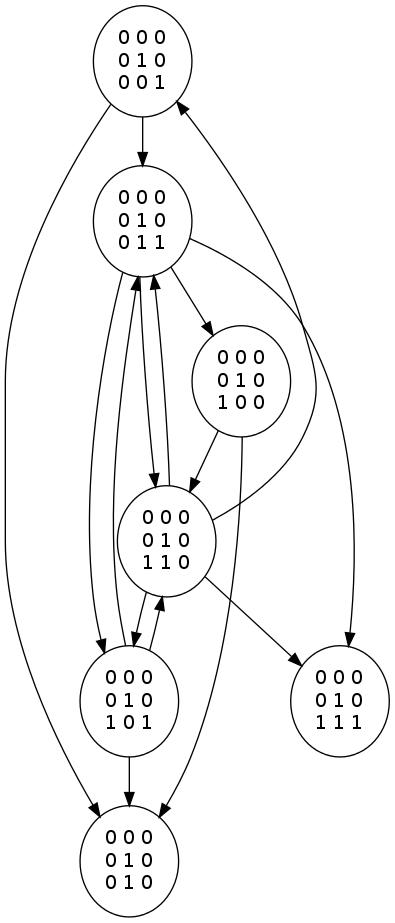
\includegraphics[scale=0.50]{body/images/graph_single_all.jpg}
  \caption{$G_{single}$}
  \label{fig:graph_single_all}
\end{figure}

\begin{figure}
  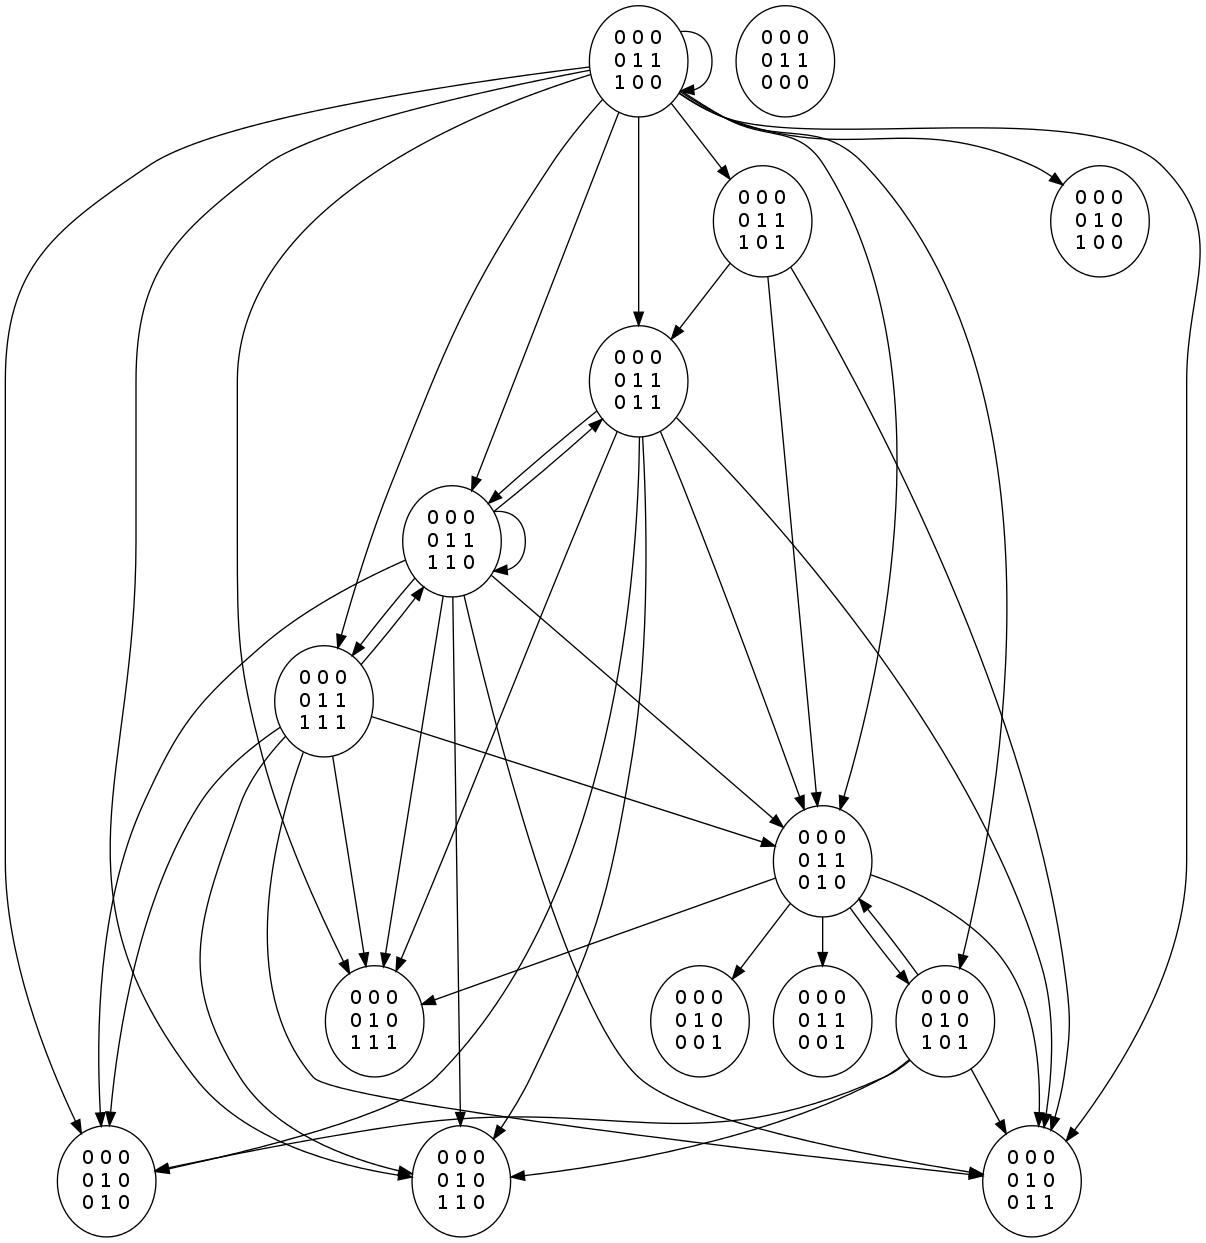
\includegraphics[scale=0.40]{body/images/graph_leftmost_mid.jpg}
  \caption{$G_{leftmost\_mid}$}
  \label{fig:graph_leftmost_mid}
\end{figure}

\begin{figure}
  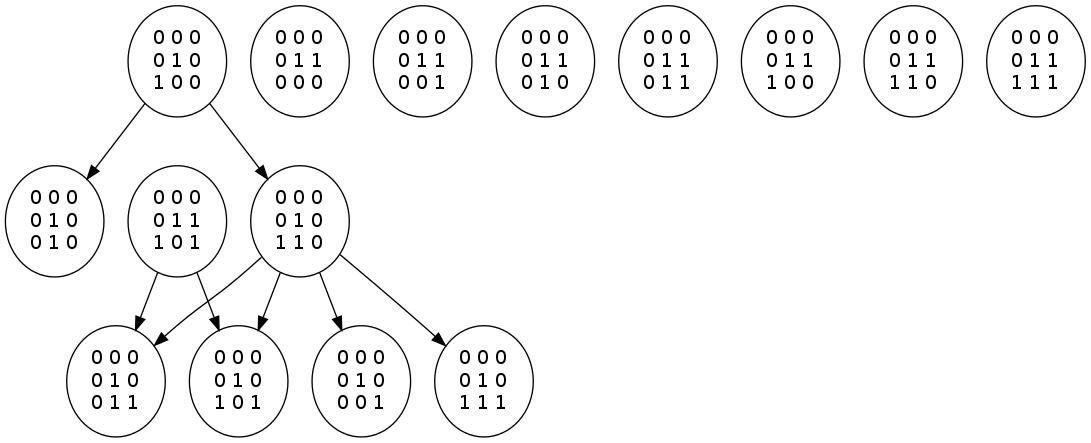
\includegraphics[scale=0.40]{body/images/graph_leftmost_left.jpg}
  \caption{$G_{leftmost\_left}$}
  \label{fig:graph_leftmost_left}
\end{figure}

\section{Cas de voisinage}

\begin{figure}[H]
  \centering
  \begin{subfigure}[b]{0.13\textwidth}
    \resizebox{\linewidth}{!} {
      \spacee {(3, 3)} {{(1, 1)}} {{}}
    }
  \end{subfigure}
  \begin{subfigure}[b]{0.13\textwidth}
    \resizebox{\linewidth}{!} {
      \spacee {(3, 3)} {{(2, 0),(1, 1)}} {{}}
    }
  \end{subfigure}
  \begin{subfigure}[b]{0.13\textwidth}
    \resizebox{\linewidth}{!} {
      \spacee {(3, 3)} {{(1, 0),(1, 1)}} {{}}
    }
  \end{subfigure}
  \begin{subfigure}[b]{0.13\textwidth}
    \resizebox{\linewidth}{!} {
      \spacee {(3, 3)} {{(2, 0),(1, 0),(1, 1)}} {{}}
    }
  \end{subfigure}
  \begin{subfigure}[b]{0.13\textwidth}
    \resizebox{\linewidth}{!} {
      \spacee {(3, 3)} {{(2, 0),(0, 0),(1, 1)}} {{}}
    }
  \end{subfigure}
  \begin{subfigure}[b]{0.13\textwidth}
    \resizebox{\linewidth}{!} {
      \spacee {(3, 3)} {{(1, 0),(0, 0),(1, 1)}} {{}}
    }
  \end{subfigure}
  \begin{subfigure}[b]{0.13\textwidth}
    \resizebox{\linewidth}{!} {
      \spacee {(3, 3)} {{(2, 0),(1, 0),(0, 0),(1, 1)}} {{}}
    }
  \end{subfigure}
  \begin{subfigure}[b]{0.13\textwidth}
    \resizebox{\linewidth}{!} {
      \spacee {(3, 3)} {{(1, 0),(2, 1),(1, 1)}} {{}}
    }
  \end{subfigure}
  \begin{subfigure}[b]{0.13\textwidth}
    \resizebox{\linewidth}{!} {
      \spacee {(3, 3)} {{(2, 0),(1, 0),(2, 1),(1, 1)}} {{}}
    }
  \end{subfigure}
  \begin{subfigure}[b]{0.13\textwidth}
    \resizebox{\linewidth}{!} {
      \spacee {(3, 3)} {{(0, 0),(2, 1),(1, 1)}} {{}}
    }
  \end{subfigure}
  \begin{subfigure}[b]{0.13\textwidth}
    \resizebox{\linewidth}{!} {
      \spacee {(3, 3)} {{(2, 0),(0, 0),(2, 1),(1, 1)}} {{}}
    }
  \end{subfigure}
  \begin{subfigure}[b]{0.13\textwidth}
    \resizebox{\linewidth}{!} {
      \spacee {(3, 3)} {{(1, 0),(0, 0),(2, 1),(1, 1)}} {{}}
    }
  \end{subfigure}
  \begin{subfigure}[b]{0.13\textwidth}
    \resizebox{\linewidth}{!} {
      \spacee {(3, 3)} {{(2, 0),(1, 0),(0, 0),(2, 1),(1, 1)}} {{}}
    }
  \end{subfigure}
  \begin{subfigure}[b]{0.13\textwidth}
    \resizebox{\linewidth}{!} {
      \spacee {(3, 3)} {{(2, 0),(1, 1),(0, 1)}} {{}}
    }
  \end{subfigure}
  \begin{subfigure}[b]{0.13\textwidth}
    \resizebox{\linewidth}{!} {
      \spacee {(3, 3)} {{(2, 0),(1, 0),(1, 1),(0, 1)}} {{}}
    }
  \end{subfigure}
  \begin{subfigure}[b]{0.13\textwidth}
    \resizebox{\linewidth}{!} {
      \spacee {(3, 3)} {{(2, 0),(0, 0),(1, 1),(0, 1)}} {{}}
    }
  \end{subfigure}
  \begin{subfigure}[b]{0.13\textwidth}
    \resizebox{\linewidth}{!} {
      \spacee {(3, 3)} {{(2, 0),(1, 0),(0, 0),(1, 1),(0, 1)}} {{}}
    }
  \end{subfigure}
  \begin{subfigure}[b]{0.13\textwidth}
    \resizebox{\linewidth}{!} {
      \spacee {(3, 3)} {{(2, 1),(1, 1),(0, 1)}} {{}}
    }
  \end{subfigure}
  \begin{subfigure}[b]{0.13\textwidth}
    \resizebox{\linewidth}{!} {
      \spacee {(3, 3)} {{(2, 0),(2, 1),(1, 1),(0, 1)}} {{}}
    }
  \end{subfigure}
  \begin{subfigure}[b]{0.13\textwidth}
    \resizebox{\linewidth}{!} {
      \spacee {(3, 3)} {{(1, 0),(2, 1),(1, 1),(0, 1)}} {{}}
    }
  \end{subfigure}
  \begin{subfigure}[b]{0.13\textwidth}
    \resizebox{\linewidth}{!} {
      \spacee {(3, 3)} {{(2, 0),(1, 0),(2, 1),(1, 1),(0, 1)}} {{}}
    }
  \end{subfigure}
  \begin{subfigure}[b]{0.13\textwidth}
    \resizebox{\linewidth}{!} {
      \spacee {(3, 3)} {{(0, 0),(2, 1),(1, 1),(0, 1)}} {{}}
    }
  \end{subfigure}
  \begin{subfigure}[b]{0.13\textwidth}
    \resizebox{\linewidth}{!} {
      \spacee {(3, 3)} {{(2, 0),(0, 0),(2, 1),(1, 1),(0, 1)}} {{}}
    }
  \end{subfigure}
  \begin{subfigure}[b]{0.13\textwidth}
    \resizebox{\linewidth}{!} {
      \spacee {(3, 3)} {{(1, 0),(0, 0),(2, 1),(1, 1),(0, 1)}} {{}}
    }
  \end{subfigure}
  \begin{subfigure}[b]{0.13\textwidth}
    \resizebox{\linewidth}{!} {
      \spacee {(3, 3)} {{(2, 0),(1, 0),(0, 0),(2, 1),(1, 1),(0, 1)}} {{}}
    }
  \end{subfigure}
  \begin{subfigure}[b]{0.13\textwidth}
    \resizebox{\linewidth}{!} {
      \spacee {(3, 3)} {{(0, 0),(1, 1),(2, 2)}} {{}}
    }
  \end{subfigure}
  \begin{subfigure}[b]{0.13\textwidth}
    \resizebox{\linewidth}{!} {
      \spacee {(3, 3)} {{(2, 0),(0, 0),(1, 1),(2, 2)}} {{}}
    }
  \end{subfigure}
  \begin{subfigure}[b]{0.13\textwidth}
    \resizebox{\linewidth}{!} {
      \spacee {(3, 3)} {{(1, 0),(0, 0),(1, 1),(2, 2)}} {{}}
    }
  \end{subfigure}
  \begin{subfigure}[b]{0.13\textwidth}
    \resizebox{\linewidth}{!} {
      \spacee {(3, 3)} {{(2, 0),(1, 0),(0, 0),(1, 1),(2, 2)}} {{}}
    }
  \end{subfigure}
  \begin{subfigure}[b]{0.13\textwidth}
    \resizebox{\linewidth}{!} {
      \spacee {(3, 3)} {{(0, 0),(2, 1),(1, 1),(2, 2)}} {{}}
    }
  \end{subfigure}
  \begin{subfigure}[b]{0.13\textwidth}
    \resizebox{\linewidth}{!} {
      \spacee {(3, 3)} {{(2, 0),(0, 0),(2, 1),(1, 1),(2, 2)}} {{}}
    }
  \end{subfigure}
  \begin{subfigure}[b]{0.13\textwidth}
    \resizebox{\linewidth}{!} {
      \spacee {(3, 3)} {{(1, 0),(0, 0),(2, 1),(1, 1),(2, 2)}} {{}}
    }
  \end{subfigure}
  \begin{subfigure}[b]{0.13\textwidth}
    \resizebox{\linewidth}{!} {
      \spacee {(3, 3)} {{(2, 0),(1, 0),(0, 0),(2, 1),(1, 1),(2, 2)}} {{}}
    }
  \end{subfigure}
  \begin{subfigure}[b]{0.13\textwidth}
    \resizebox{\linewidth}{!} {
      \spacee {(3, 3)} {{(2, 0),(1, 1),(0, 1),(2, 2)}} {{}}
    }
  \end{subfigure}
  \begin{subfigure}[b]{0.13\textwidth}
    \resizebox{\linewidth}{!} {
      \spacee {(3, 3)} {{(1, 0),(1, 1),(0, 1),(2, 2)}} {{}}
    }
  \end{subfigure}
  \begin{subfigure}[b]{0.13\textwidth}
    \resizebox{\linewidth}{!} {
      \spacee {(3, 3)} {{(2, 0),(1, 0),(1, 1),(0, 1),(2, 2)}} {{}}
    }
  \end{subfigure}
  \begin{subfigure}[b]{0.13\textwidth}
    \resizebox{\linewidth}{!} {
      \spacee {(3, 3)} {{(2, 0),(0, 0),(1, 1),(0, 1),(2, 2)}} {{}}
    }
  \end{subfigure}
  \begin{subfigure}[b]{0.13\textwidth}
    \resizebox{\linewidth}{!} {
      \spacee {(3, 3)} {{(1, 0),(0, 0),(1, 1),(0, 1),(2, 2)}} {{}}
    }
  \end{subfigure}
  \begin{subfigure}[b]{0.13\textwidth}
    \resizebox{\linewidth}{!} {
      \spacee {(3, 3)} {{(2, 0),(1, 0),(0, 0),(1, 1),(0, 1),(2, 2)}} {{}}
    }
  \end{subfigure}
  \begin{subfigure}[b]{0.13\textwidth}
    \resizebox{\linewidth}{!} {
      \spacee {(3, 3)} {{(2, 0),(2, 1),(1, 1),(0, 1),(2, 2)}} {{}}
    }
  \end{subfigure}
  \begin{subfigure}[b]{0.13\textwidth}
    \resizebox{\linewidth}{!} {
      \spacee {(3, 3)} {{(1, 0),(2, 1),(1, 1),(0, 1),(2, 2)}} {{}}
    }
  \end{subfigure}
  \begin{subfigure}[b]{0.13\textwidth}
    \resizebox{\linewidth}{!} {
      \spacee {(3, 3)} {{(2, 0),(1, 0),(2, 1),(1, 1),(0, 1),(2, 2)}} {{}}
    }
  \end{subfigure}
  \begin{subfigure}[b]{0.13\textwidth}
    \resizebox{\linewidth}{!} {
      \spacee {(3, 3)} {{(0, 0),(2, 1),(1, 1),(0, 1),(2, 2)}} {{}}
    }
  \end{subfigure}
  \begin{subfigure}[b]{0.13\textwidth}
    \resizebox{\linewidth}{!} {
      \spacee {(3, 3)} {{(2, 0),(0, 0),(2, 1),(1, 1),(0, 1),(2, 2)}} {{}}
    }
  \end{subfigure}
  \begin{subfigure}[b]{0.13\textwidth}
    \resizebox{\linewidth}{!} {
      \spacee {(3, 3)} {{(1, 0),(0, 0),(2, 1),(1, 1),(0, 1),(2, 2)}} {{}}
    }
  \end{subfigure}
  \begin{subfigure}[b]{0.13\textwidth}
    \resizebox{\linewidth}{!} {
      \spacee {(3, 3)} {{(2, 0),(1, 0),(0, 0),(2, 1),(1, 1),(0, 1),(2, 2)}} {{}}
    }
  \end{subfigure}
  \begin{subfigure}[b]{0.13\textwidth}
    \resizebox{\linewidth}{!} {
      \spacee {(3, 3)} {{(2, 0),(0, 0),(2, 1),(1, 1),(1, 2)}} {{}}
    }
  \end{subfigure}
  \begin{subfigure}[b]{0.13\textwidth}
    \resizebox{\linewidth}{!} {
      \spacee {(3, 3)} {{(1, 0),(0, 0),(2, 1),(1, 1),(1, 2)}} {{}}
    }
  \end{subfigure}
  \begin{subfigure}[b]{0.13\textwidth}
    \resizebox{\linewidth}{!} {
      \spacee {(3, 3)} {{(2, 0),(1, 0),(0, 0),(2, 1),(1, 1),(1, 2)}} {{}}
    }
  \end{subfigure}
  \begin{subfigure}[b]{0.13\textwidth}
    \resizebox{\linewidth}{!} {
      \spacee {(3, 3)} {{(1, 0),(2, 1),(1, 1),(0, 1),(1, 2)}} {{}}
    }
  \end{subfigure}
  \begin{subfigure}[b]{0.13\textwidth}
    \resizebox{\linewidth}{!} {
      \spacee {(3, 3)} {{(2, 0),(1, 0),(2, 1),(1, 1),(0, 1),(1, 2)}} {{}}
    }
  \end{subfigure}
  \begin{subfigure}[b]{0.13\textwidth}
    \resizebox{\linewidth}{!} {
      \spacee {(3, 3)} {{(2, 0),(0, 0),(2, 1),(1, 1),(0, 1),(1, 2)}} {{}}
    }
  \end{subfigure}
  \begin{subfigure}[b]{0.13\textwidth}
    \resizebox{\linewidth}{!} {
      \spacee {(3, 3)} {{(2, 0),(1, 0),(0, 0),(2, 1),(1, 1),(0, 1),(1, 2)}} {{}}
    }
  \end{subfigure}
  \begin{subfigure}[b]{0.13\textwidth}
    \resizebox{\linewidth}{!} {
      \spacee {(3, 3)} {{(2, 0),(0, 0),(1, 1),(2, 2),(1, 2)}} {{}}
    }
  \end{subfigure}
  \begin{subfigure}[b]{0.13\textwidth}
    \resizebox{\linewidth}{!} {
      \spacee {(3, 3)} {{(1, 0),(0, 0),(1, 1),(2, 2),(1, 2)}} {{}}
    }
  \end{subfigure}
  \begin{subfigure}[b]{0.13\textwidth}
    \resizebox{\linewidth}{!} {
      \spacee {(3, 3)} {{(2, 0),(1, 0),(0, 0),(1, 1),(2, 2),(1, 2)}} {{}}
    }
  \end{subfigure}
  \begin{subfigure}[b]{0.13\textwidth}
    \resizebox{\linewidth}{!} {
      \spacee {(3, 3)} {{(2, 0),(0, 0),(2, 1),(1, 1),(2, 2),(1, 2)}} {{}}
    }
  \end{subfigure}
  \begin{subfigure}[b]{0.13\textwidth}
    \resizebox{\linewidth}{!} {
      \spacee {(3, 3)} {{(1, 0),(0, 0),(2, 1),(1, 1),(2, 2),(1, 2)}} {{}}
    }
  \end{subfigure}
  \begin{subfigure}[b]{0.13\textwidth}
    \resizebox{\linewidth}{!} {
      \spacee {(3, 3)} {{(2, 0),(1, 0),(0, 0),(2, 1),(1, 1),(2, 2),(1, 2)}} {{}}
    }
  \end{subfigure}
  \begin{subfigure}[b]{0.13\textwidth}
    \resizebox{\linewidth}{!} {
      \spacee {(3, 3)} {{(2, 0),(0, 0),(1, 1),(0, 1),(2, 2),(1, 2)}} {{}}
    }
  \end{subfigure}
  \begin{subfigure}[b]{0.13\textwidth}
    \resizebox{\linewidth}{!} {
      \spacee {(3, 3)} {{(2, 0),(1, 0),(0, 0),(1, 1),(0, 1),(2, 2),(1, 2)}} {{}}
    }
  \end{subfigure}
  \begin{subfigure}[b]{0.13\textwidth}
    \resizebox{\linewidth}{!} {
      \spacee {(3, 3)} {{(2, 0),(0, 0),(2, 1),(1, 1),(0, 1),(2, 2),(1, 2)}} {{}}
    }
  \end{subfigure}
  \begin{subfigure}[b]{0.13\textwidth}
    \resizebox{\linewidth}{!} {
      \spacee {(3, 3)} {{(1, 0),(0, 0),(2, 1),(1, 1),(0, 1),(2, 2),(1, 2)}} {{}}
    }
  \end{subfigure}
  \begin{subfigure}[b]{0.13\textwidth}
    \resizebox{\linewidth}{!} {
      \spacee {(3, 3)} {{(2, 0),(1, 0),(0, 0),(2, 1),(1, 1),(0, 1),(2, 2),(1, 2)}} {{}}
    }
  \end{subfigure}
  \begin{subfigure}[b]{0.13\textwidth}
    \resizebox{\linewidth}{!} {
      \spacee {(3, 3)} {{(2, 0),(0, 0),(1, 1),(2, 2),(0, 2)}} {{}}
    }
  \end{subfigure}
  \begin{subfigure}[b]{0.13\textwidth}
    \resizebox{\linewidth}{!} {
      \spacee {(3, 3)} {{(2, 0),(1, 0),(0, 0),(1, 1),(2, 2),(0, 2)}} {{}}
    }
  \end{subfigure}
  \begin{subfigure}[b]{0.13\textwidth}
    \resizebox{\linewidth}{!} {
      \spacee {(3, 3)} {{(2, 0),(1, 0),(0, 0),(2, 1),(1, 1),(2, 2),(0, 2)}} {{}}
    }
  \end{subfigure}
  \begin{subfigure}[b]{0.13\textwidth}
    \resizebox{\linewidth}{!} {
      \spacee {(3, 3)} {{(2, 0),(0, 0),(2, 1),(1, 1),(0, 1),(2, 2),(0, 2)}} {{}}
    }
  \end{subfigure}
  \begin{subfigure}[b]{0.13\textwidth}
    \resizebox{\linewidth}{!} {
      \spacee {(3, 3)} {{(2, 0),(1, 0),(0, 0),(2, 1),(1, 1),(0, 1),(2, 2),(0, 2)}} {{}}
    }
  \end{subfigure}
  \begin{subfigure}[b]{0.13\textwidth}
    \resizebox{\linewidth}{!} {
      \spacee {(3, 3)} {{(2, 0),(1, 0),(0, 0),(2, 1),(1, 1),(0, 1),(2, 2),(1, 2),(0, 2)}} {{}}
    }
  \end{subfigure}
  \caption{Tous les cas de voisinnage}
  \label{fig:cas}
\end{figure}


\section{Capture d'écran}

\begin{figure}[H]
  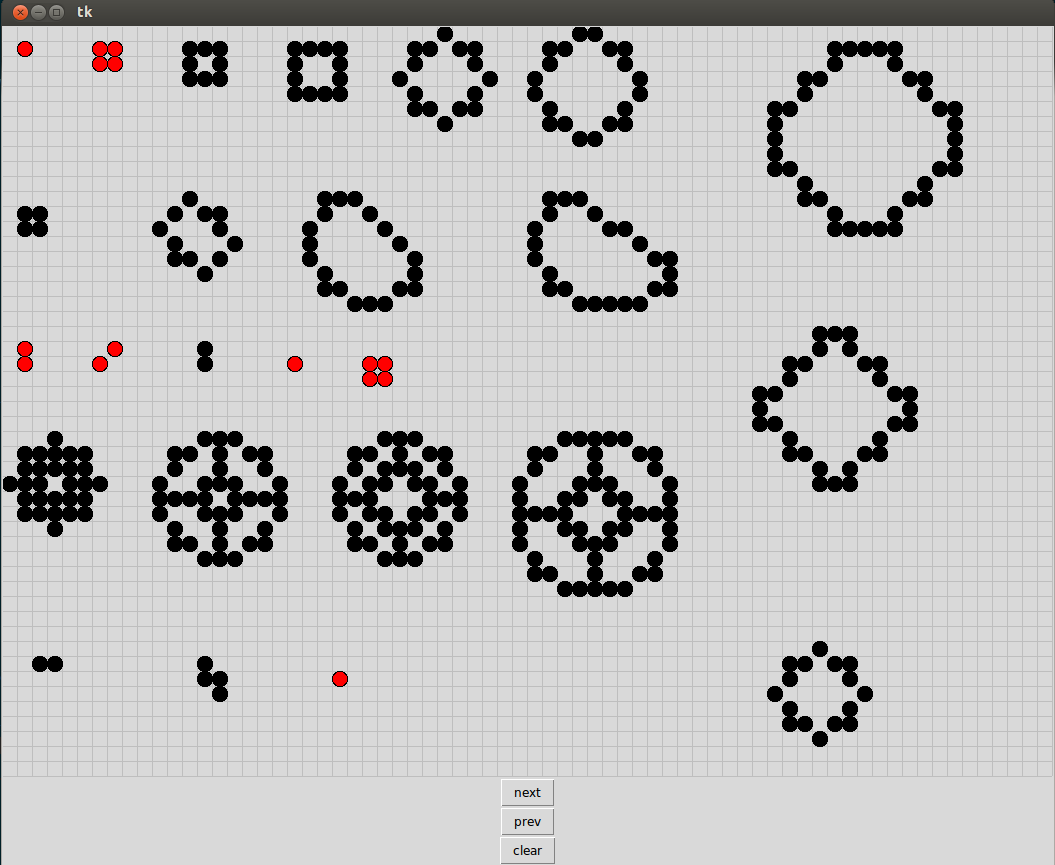
\includegraphics[scale=0.50]{body/images/screenshot.png}
  \caption{Capture d'écran de l'application}
  \label{fig:screenshot}
\end{figure}



\end{document}
